% Teorema
\begin{frame}
    \frametitle{El problema.}    
    \begin{teorema} %%Uso del "environment" definido al inicio del documento.
      Sean $\alpha_1, \alpha_2, \alpha_3$ tres ángulos tales que
      \[\alpha_1 + \alpha_2 + \alpha_3 = \pi\]
      y sea $P$ un polígono convexo. Entonces siempre podemos colocar tres reflectores
      de tamaño a lo más $\alpha_1, \alpha_2, \alpha_3$ con ápices sobre vértices de $P$
      de manera que $P$ quede iluminado, y no coloquemos más de un reflector sobre cada
      vértice de $P$.
    \end{teorema}
\end{frame}

% Demostración:
\begin{frame}
    \frametitle{Prueba.}    
    Es fácil ver que un triángulo cumple con el teorema. Supongamos $P$ un polígono convexo con al menos $4$
    vértices.\newline

    Supongamos que $\alpha_1 \leq \alpha_2 \leq \alpha_3 \Rightarrow \alpha_2 < \frac{\pi}{2}$.  Además, cómo
    $P$ tiene al menos $4$ vértices entonces al menos uno de los ángulos generados por sus vértices es mayor
    o igual que $\frac{\pi}{2}$. Sea $T$ un triángulo cuyos ángulos sean $\alpha_1, \alpha_2,$ y $\alpha_3$
    tal que:
    \begin{enumerate}
    \item El vértice de $T$ de tamaño $\alpha_2$ está colocado sobre un vértice $v$ de $P$ que genera un ángulo
      mayor o igual a $\alpha_2$.
    \item Los otros dos vértices de $T$ están colocados sobre dos puntos $x, y$ en la frontera de $P$.
    \end{enumerate}
    Supongamos que $x,y$ pertenecen a aristas distintas en $P$.
\end{frame}

\begin{frame}
  \frametitle{Prueba.}
  Análicemos dos posibles casos:
  \begin{enumerate}
  \item $u \not= w$. Coloquemos un reflector $f_1$ sobre $u$ iluminando la zona angular
    determinada por $v, u, x$ y otro, $f_3$ sobre $w$ iluminado la zona angular
    determinada por $v, w, y$. Como $f_1$ y $f_3$ no están en el interior de $C$, los
    angulos de iluminación de $f_1$ y $f_3$ son a lo más, $\alpha_1$ y $\alpha_2$ respectivamente.
  \item $u = w$. Sea $T'$ el triángulo determinado por el segmento que une a $x$ con
    $y$, y las tangentes a $C$ en estos puntos. El ángulo generado en el vértice
    $z$ de $T'$  que no está sobre $C$ es $\pi - 2\alpha_2$. Nótese que $z$ pertenece al interior
    del triángulo $T''$ con vértices $x, y, u$ y por tanto el ángulo de $T''$ en $u$ es
    menor que $\pi - 2\alpha_2$. Como $\alpha \leq \alpha_2 \leq \alpha_3 \leq \pi - 2\alpha_2 \leq (\pi - (\alpha_1 + \alpha_2)) = \alpha_3$.
    Por tanto colocando un reflector de tamaño a lo más $\alpha_3$ en u iluminamos P.
  \end{enumerate}
\end{frame}


{\setbeamertemplate{background}{

\includegraphics[width=\the\paperwidth,height=\the\paperheight]{images/White.png}}

\begin{frame}
  \frametitle{Caso 1.}
  \begin{figure}
    \centering
    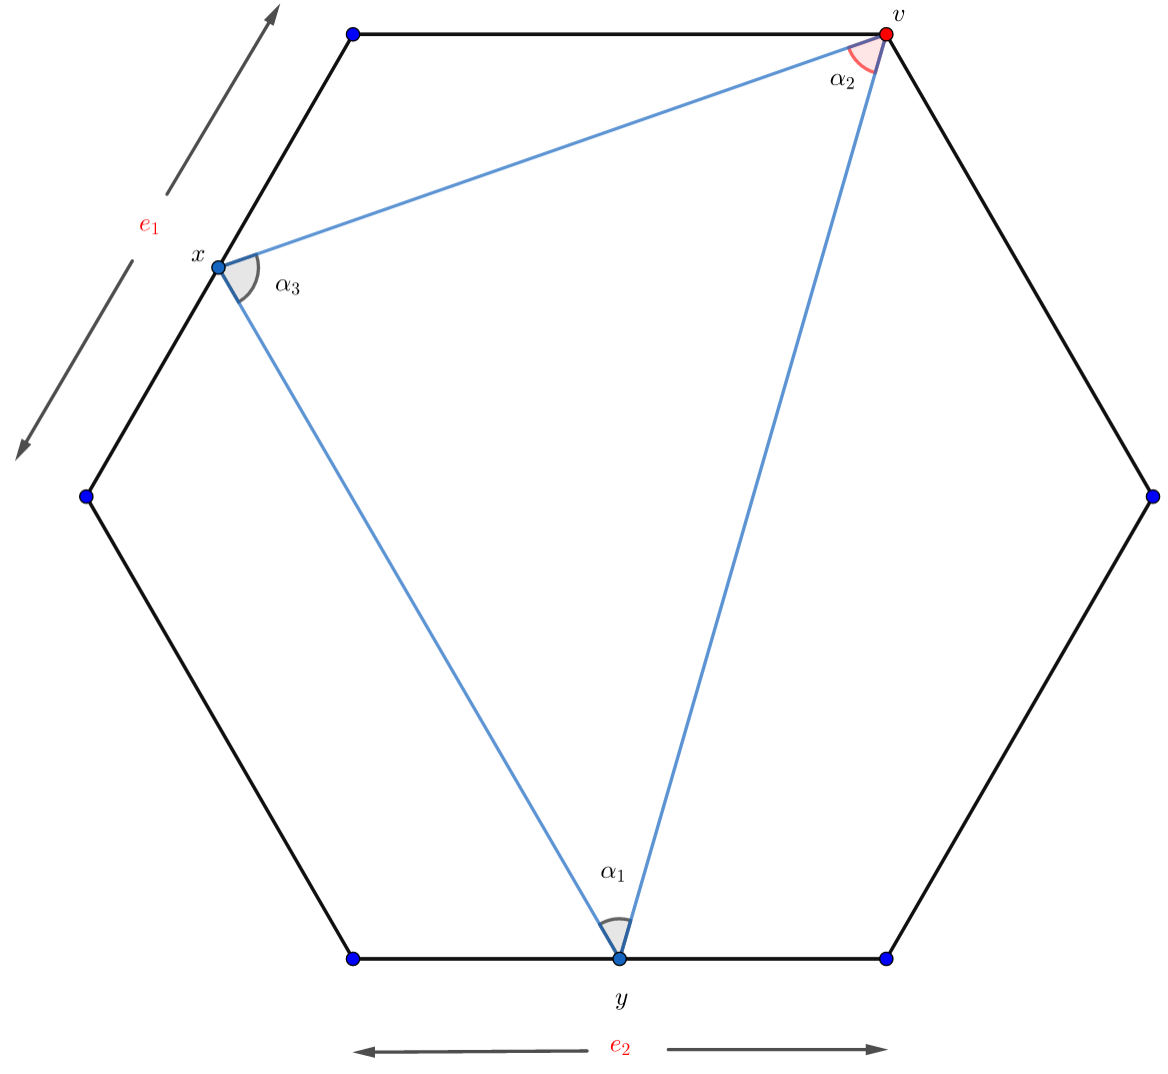
\includegraphics[width=.50 \paperwidth]{./images/Bosquejo1.png}
    %\caption*{.}
  \end{figure}
\end{frame}

\begin{frame}
  %\frametitle{Prueba.}
  \begin{figure}
    \centering
    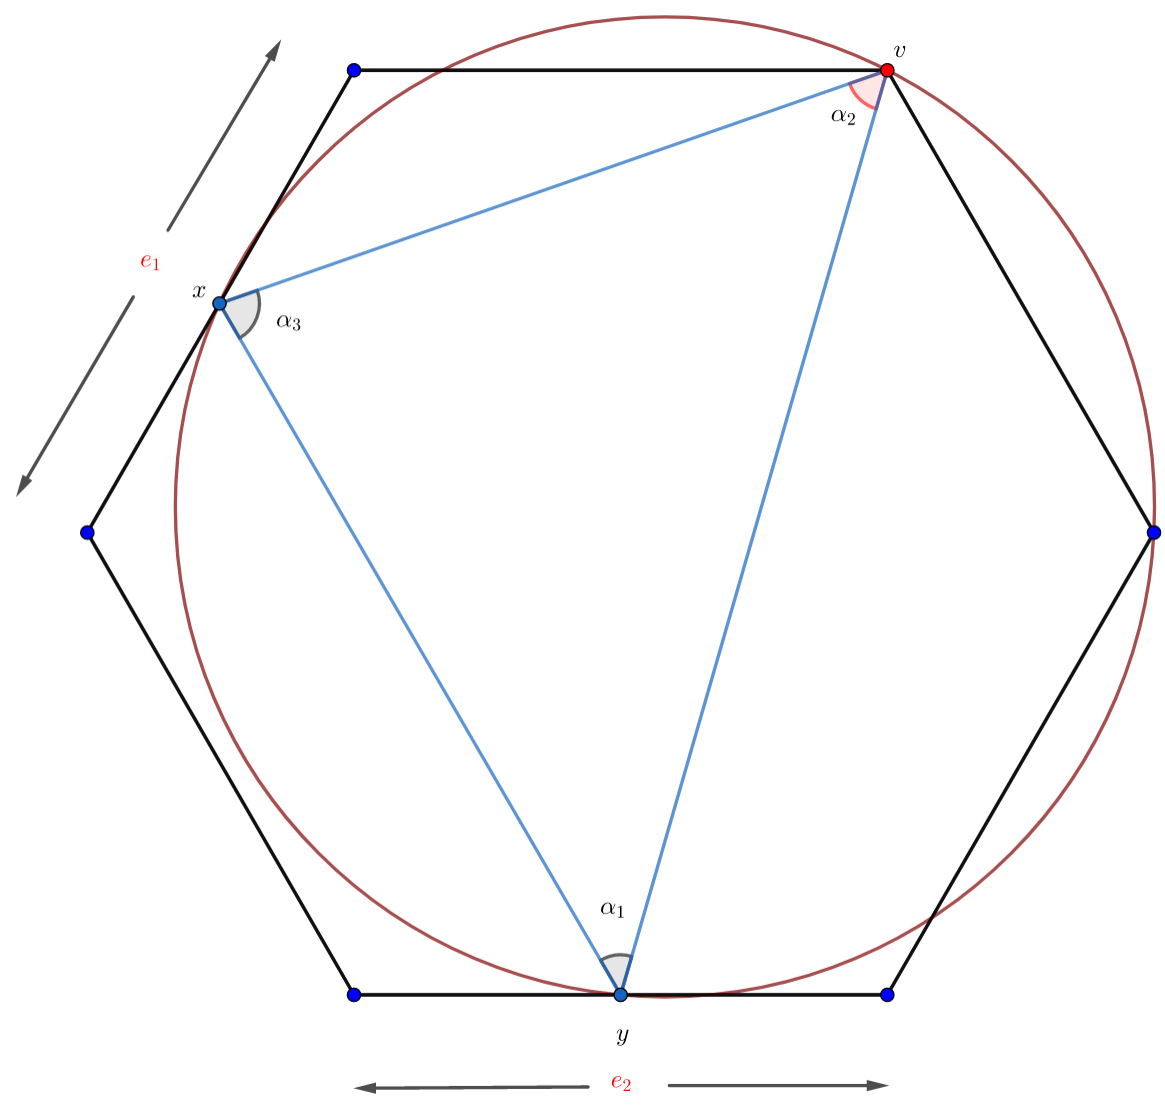
\includegraphics[width=.65 \paperwidth]{./images/Bosquejo2.png}
    %\caption*{.}
  \end{figure}
\end{frame}

\begin{frame}
  %\frametitle{Prueba.}
  \begin{figure}
    \centering
    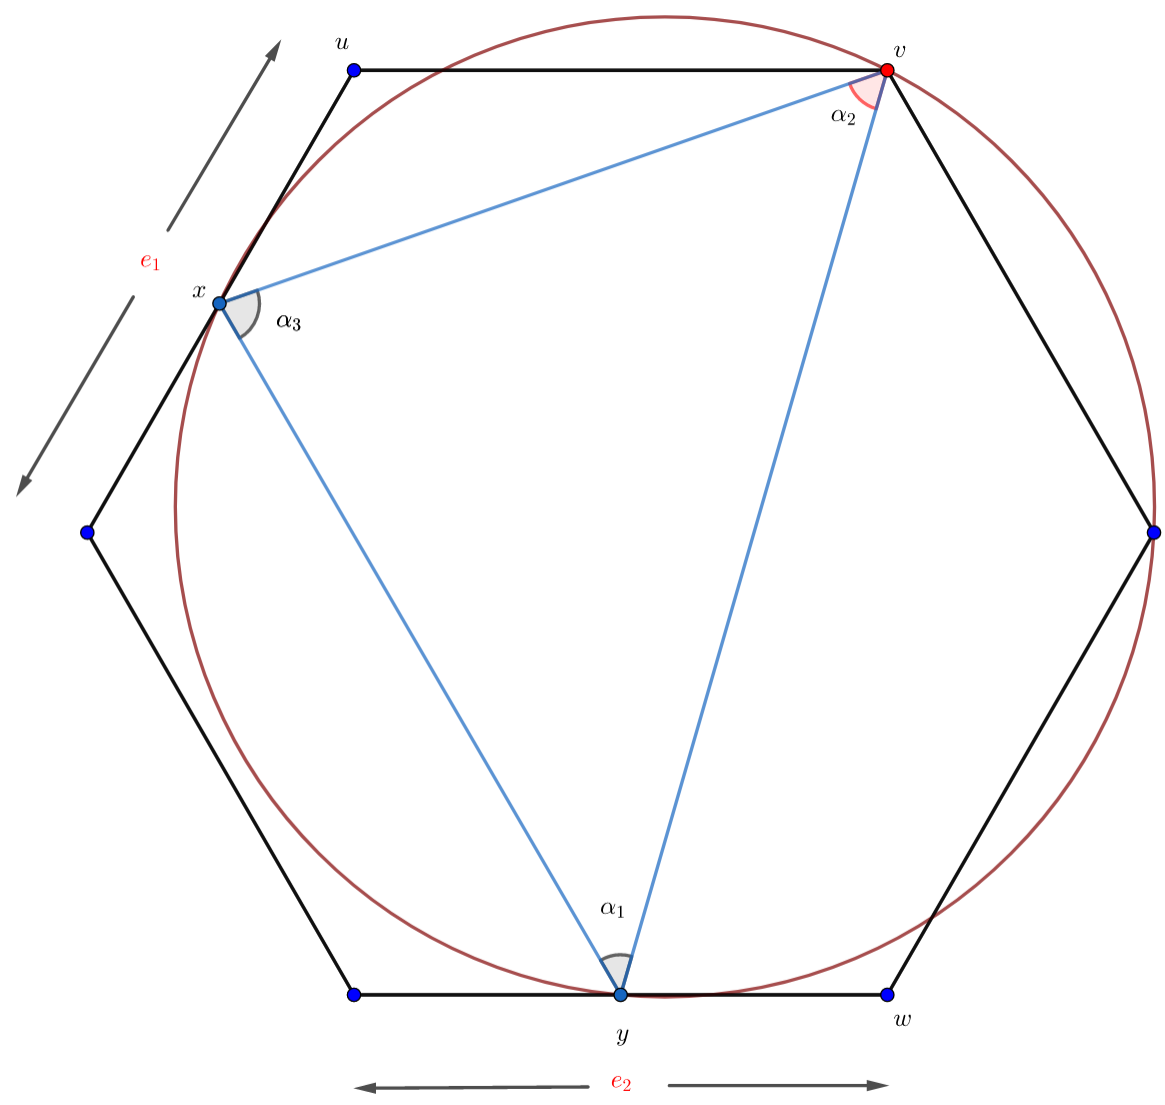
\includegraphics[width=.65 \paperwidth]{./images/Bosquejo3.png}
    %\caption*{.}
  \end{figure}
\end{frame}

\begin{frame}
  %\frametitle{Prueba.}
  \begin{figure}
    \centering
    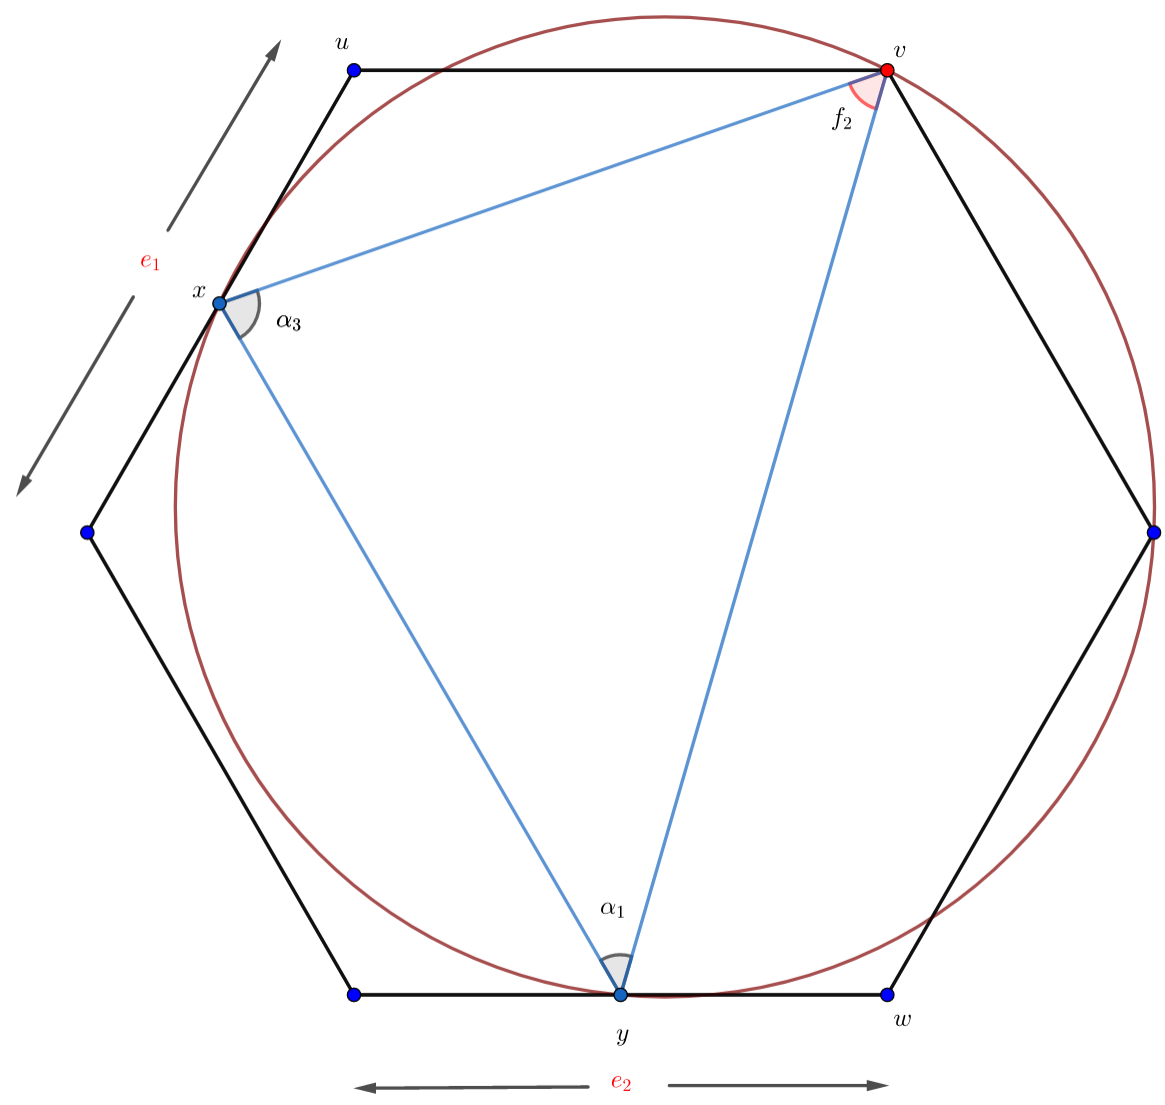
\includegraphics[width=.65 \paperwidth]{./images/Bosquejo4.png}
    %\caption*{.}
  \end{figure}
\end{frame}

\begin{frame}
  %\frametitle{Prueba.}
  \begin{figure}
    \centering
    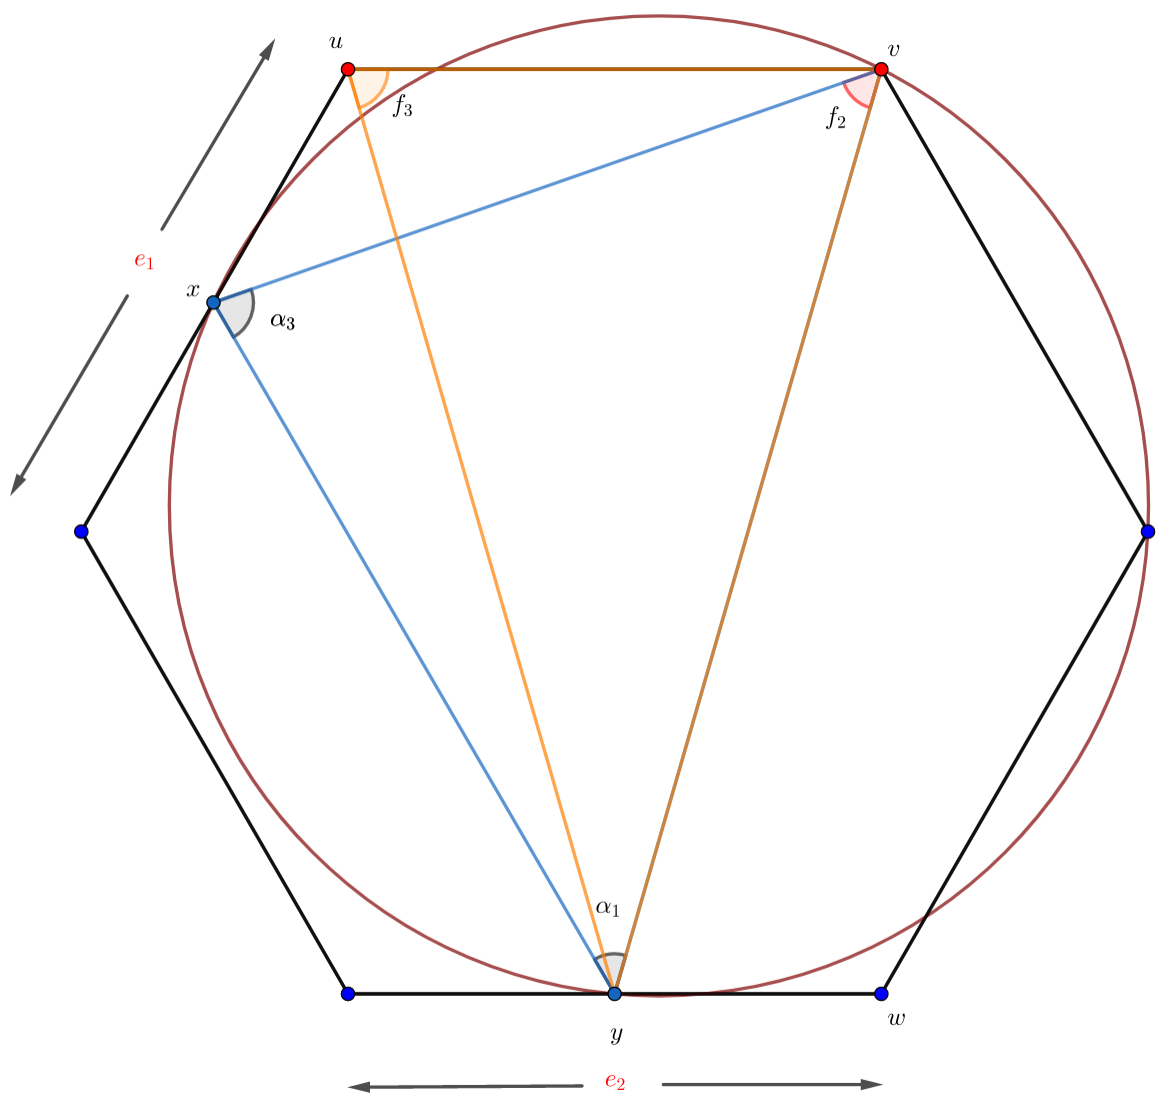
\includegraphics[width=.65 \paperwidth]{./images/Bosquejo5.png}
    %\caption*{.}
  \end{figure}
\end{frame}

\begin{frame}
  %\frametitle{Prueba.}
  \begin{figure}
    \centering
    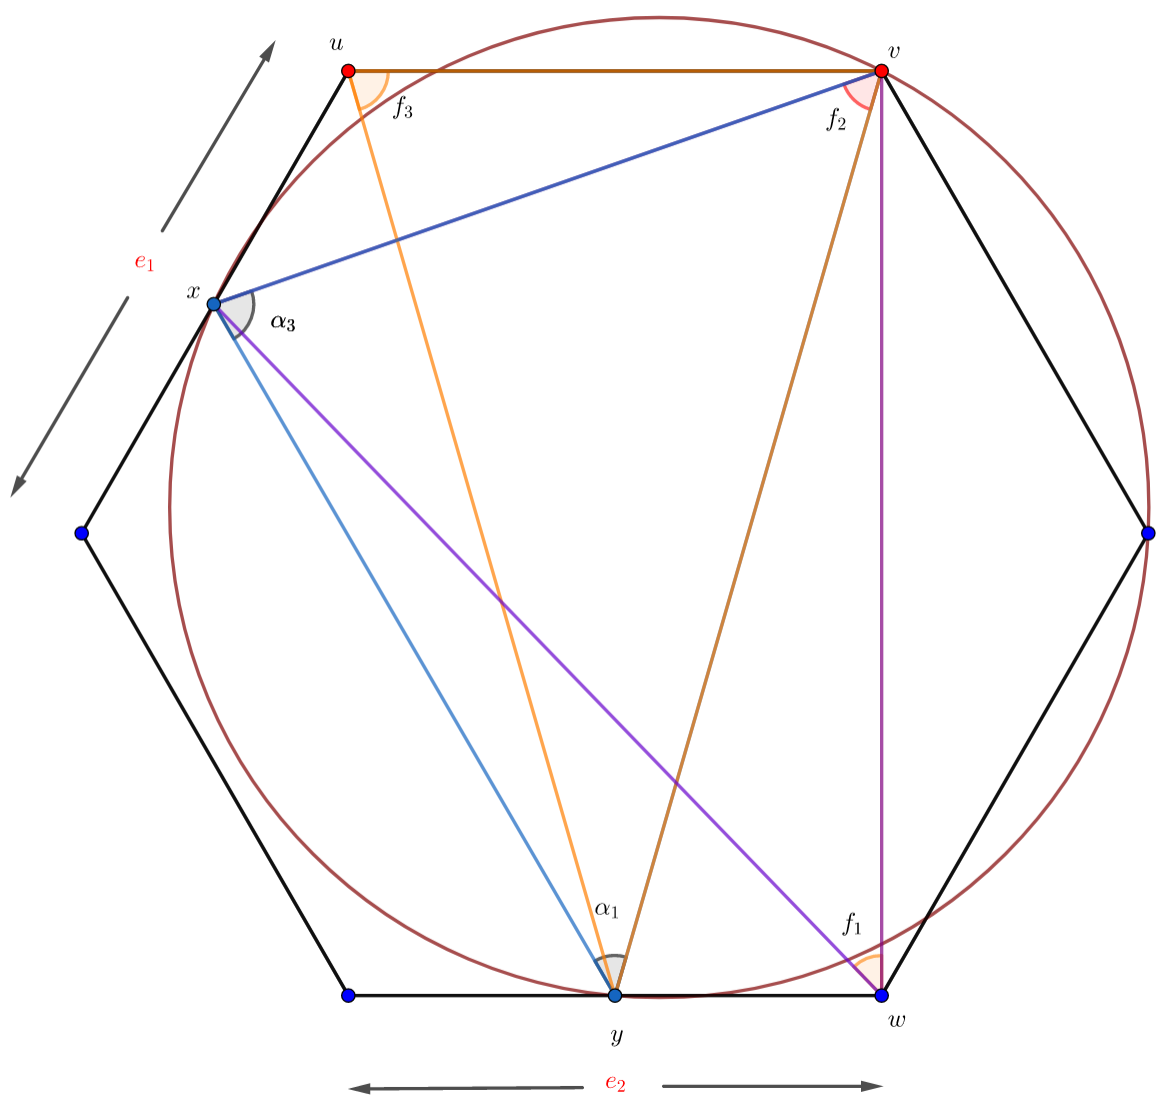
\includegraphics[width=.65 \paperwidth]{./images/Bosquejo6.png}
    %\caption*{.}
  \end{figure}
\end{frame} 

\begin{frame}
  %\frametitle{Prueba.}
  \begin{figure}
    \centering
    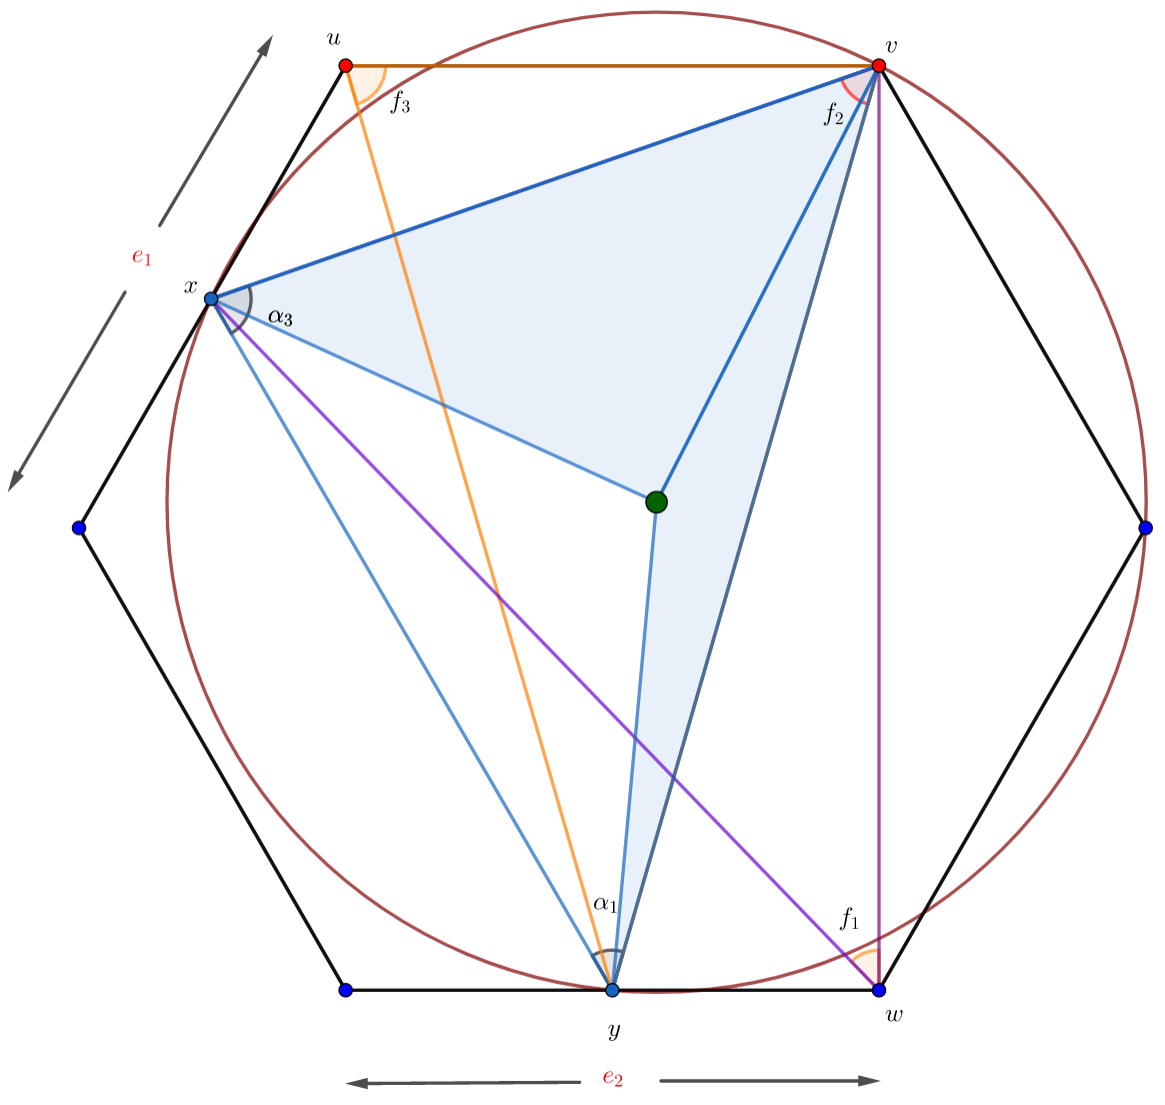
\includegraphics[width=.65 \paperwidth]{./images/Bosquejo7.png}
    %\caption*{.}
  \end{figure}
\end{frame} 

\begin{frame}
  %\frametitle{Prueba.}
  \begin{figure}
    \centering
    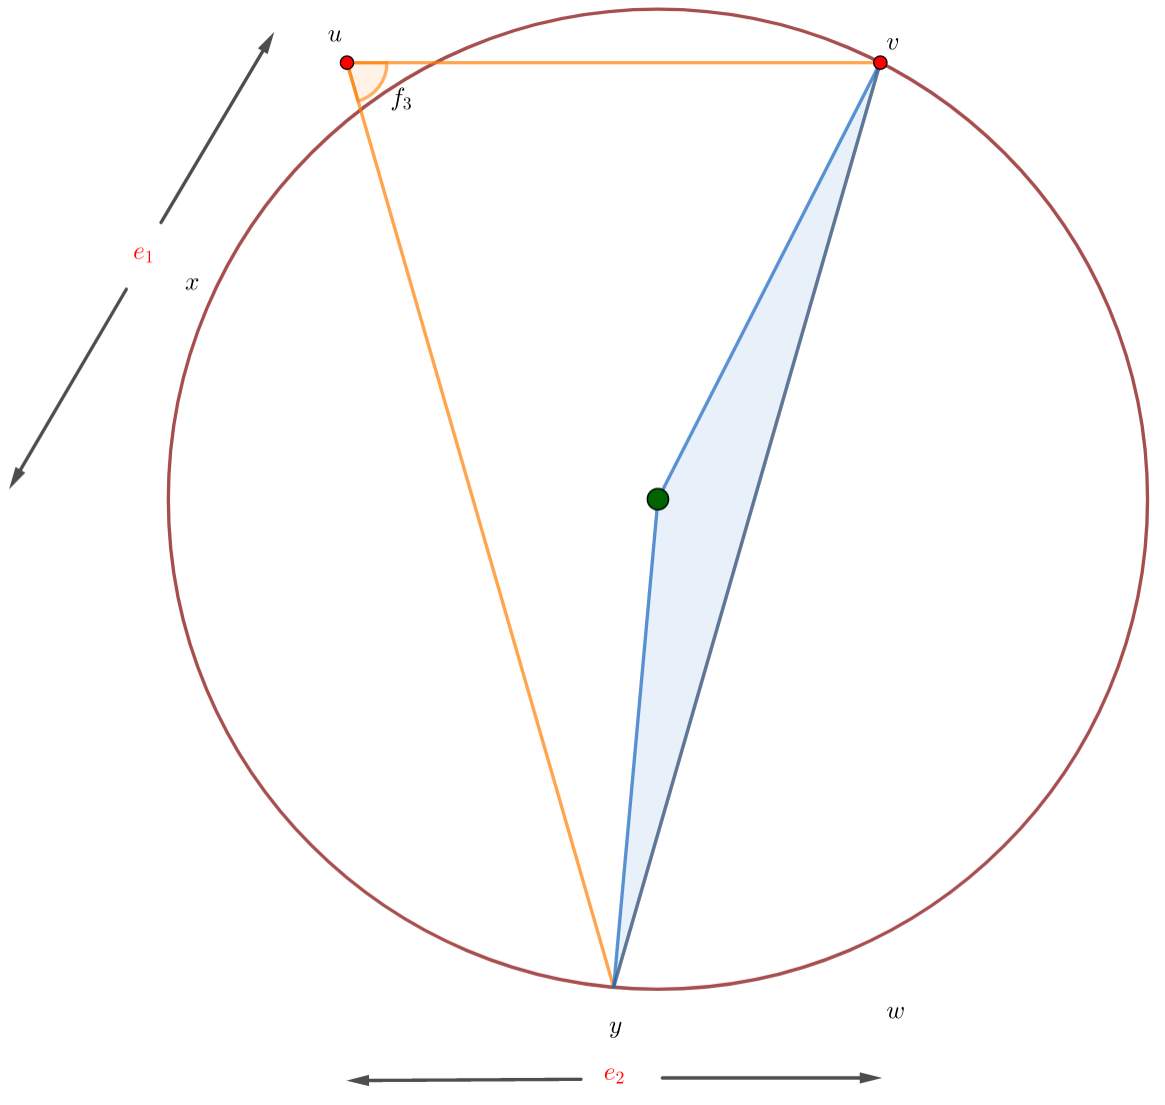
\includegraphics[width=.65 \paperwidth]{./images/Bosquejo8.png}
    %\caption*{.}
  \end{figure}
\end{frame} 

\begin{frame}
  %\frametitle{Prueba.}
  \begin{figure}
    \centering
    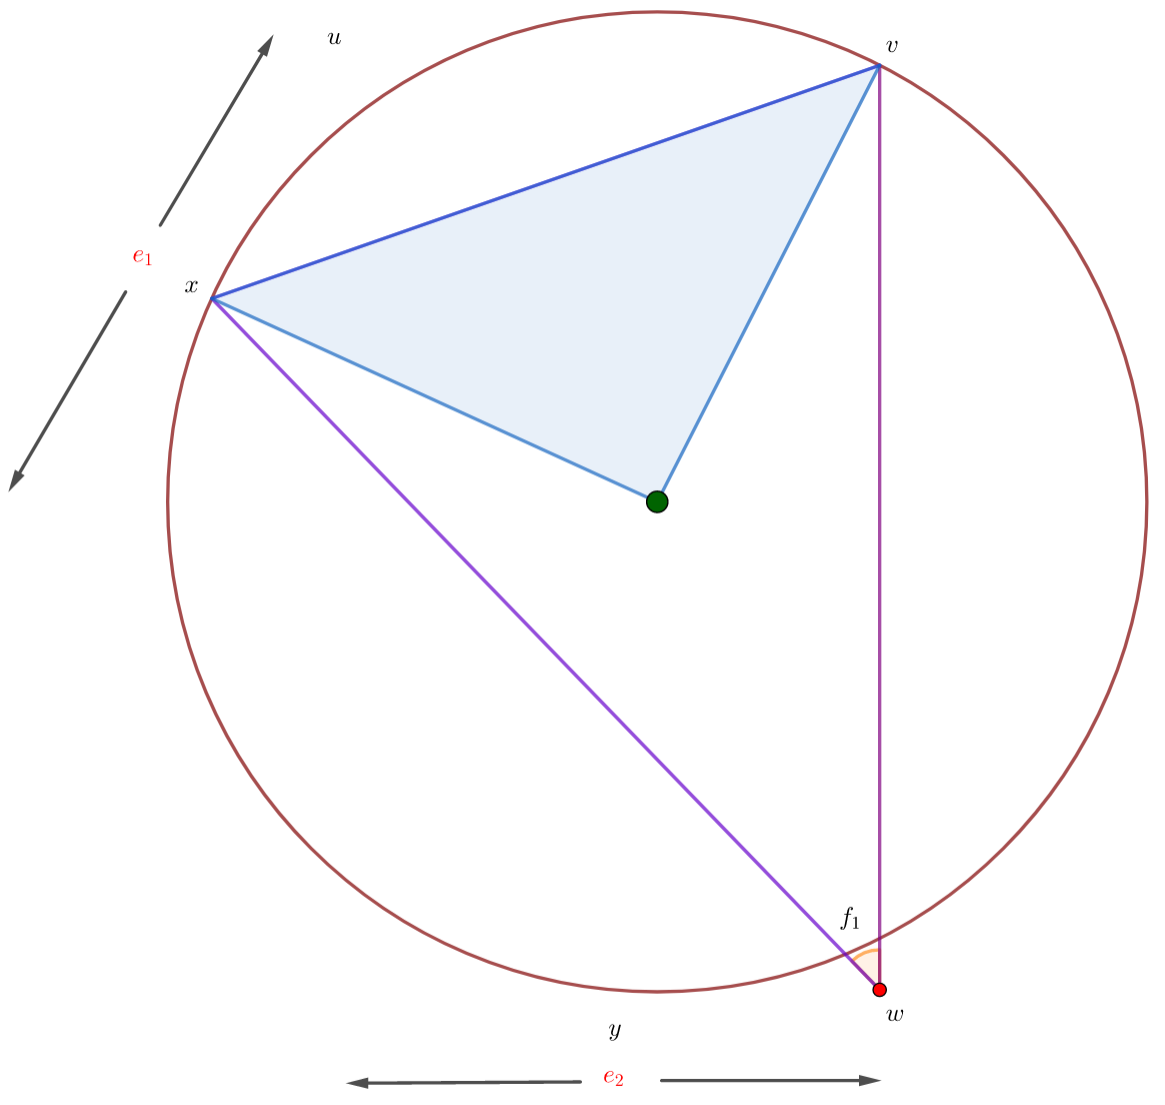
\includegraphics[width=.65 \paperwidth]{./images/Bosquejo9.png}
    %\caption*{.}
  \end{figure}
\end{frame} 

\begin{frame}
  %\frametitle{Prueba.}
  \begin{figure}
    \centering
    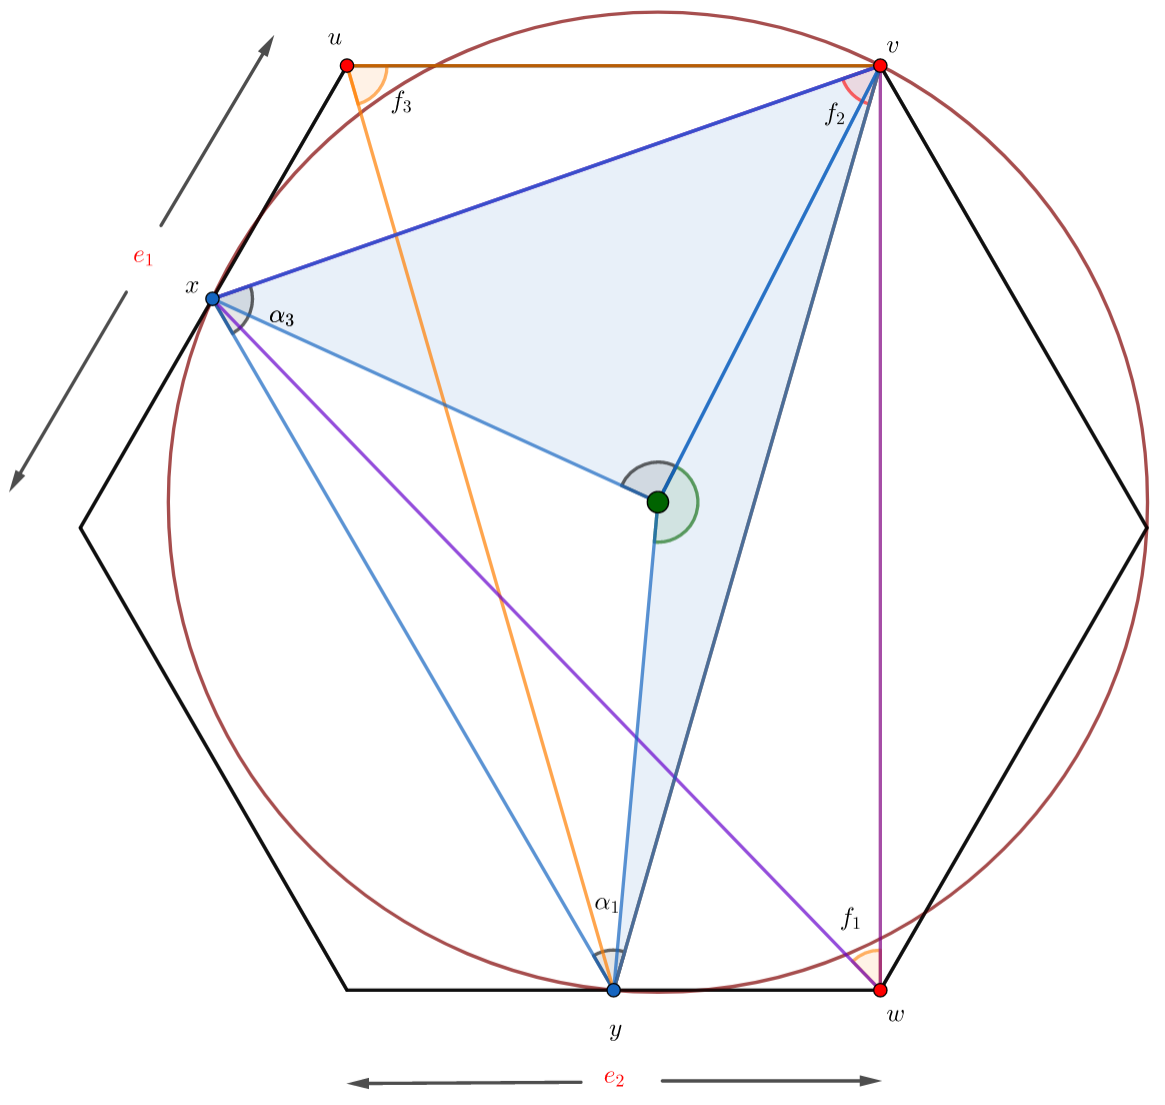
\includegraphics[width=.65 \paperwidth]{./images/Bosquejo10.png}
    %\caption*{.}
  \end{figure}
\end{frame} 

\begin{frame}
  \frametitle{Cuentas ...}
  Primero observemos que
  \begin{eqnarray*}
    \sphericalangle vox &=& 2 \alpha_1\\
    \sphericalangle voy &=& 2 \alpha_3
  \end{eqnarray*}
  Luego, tenemos que
 \begin{eqnarray*}
    f_1 &=& \frac{2\alpha_1 - \sphericalangle x'}{2}\\
    f_3 &=& \frac{2\alpha_3 - \sphericalangle y'}{2}
  \end{eqnarray*}
 En partícular, se cumple que
 \begin{eqnarray*}
    f_1 + f_3 &=& \frac{2\alpha_1 - \sphericalangle x'}{2} +  \frac{2\alpha_3 - \sphericalangle y'}{2}\\
              &=& \alpha_1 + \alpha_3 - \frac{\sphericalangle x' + \sphericalangle y'}{2}
 \end{eqnarray*}

 .\newline

 .
\end{frame} 


\begin{frame}
  %\frametitle{Prueba.}
  \begin{figure}
    \centering
    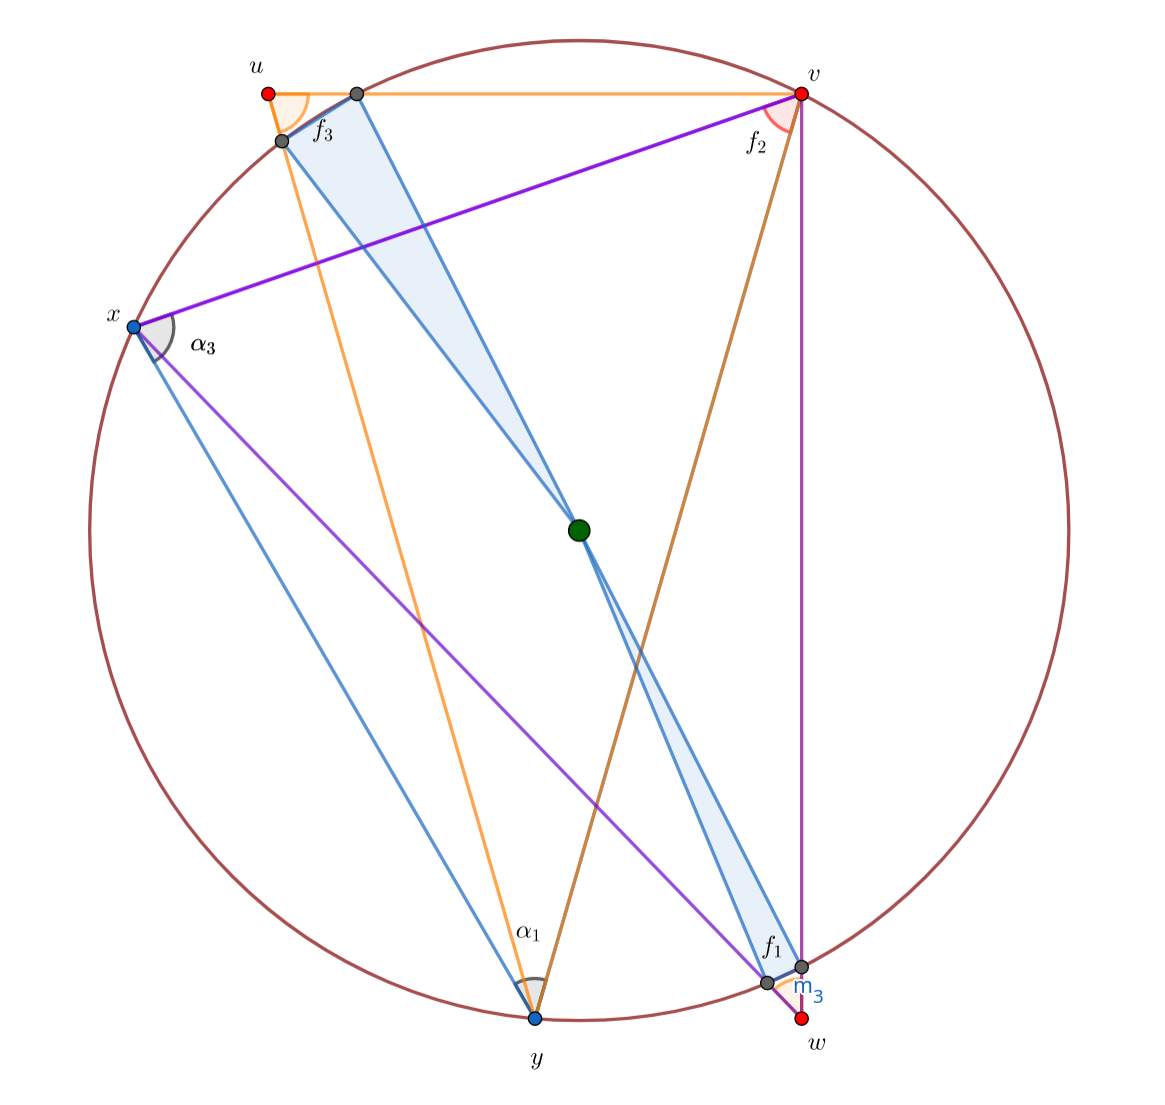
\includegraphics[width=.65 \paperwidth]{./images/Bosquejo11.png}
    %\caption*{.}
  \end{figure}
\end{frame} 

\begin{frame}
  %\frametitle{Prueba.}
  \begin{figure}
    \centering
    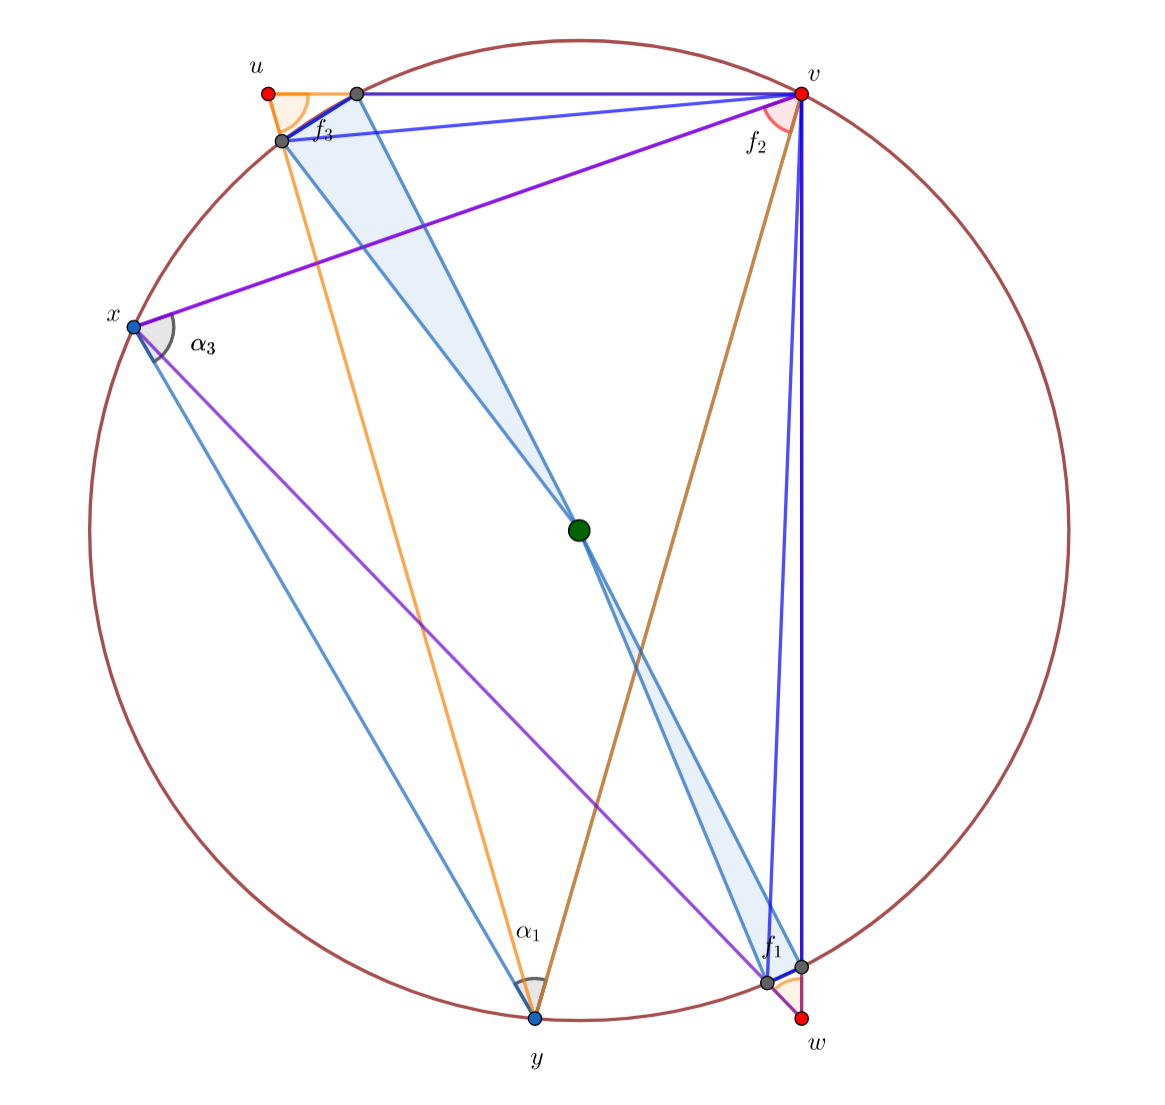
\includegraphics[width=.65 \paperwidth]{./images/Bosquejo12.png}
    %\caption*{.}
  \end{figure}
\end{frame} 

\begin{frame}
  %\frametitle{Prueba.}
  \begin{figure}
    \centering
    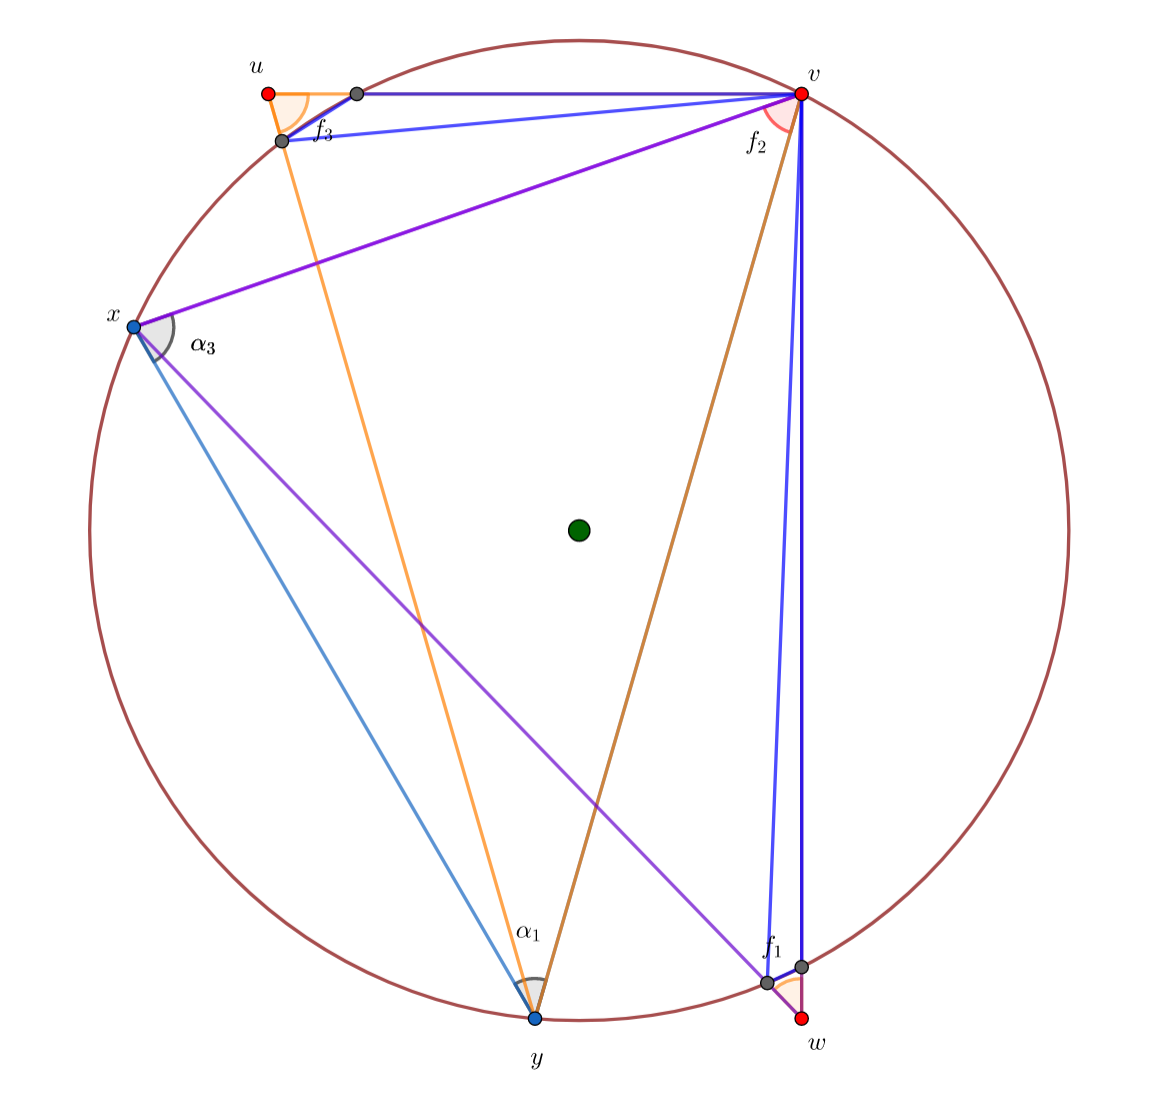
\includegraphics[width=.65 \paperwidth]{./images/Bosquejo13.png}
    %\caption*{.}
  \end{figure}
\end{frame} 

\begin{frame}
  %\frametitle{Prueba.}
  \begin{figure}
    \centering
    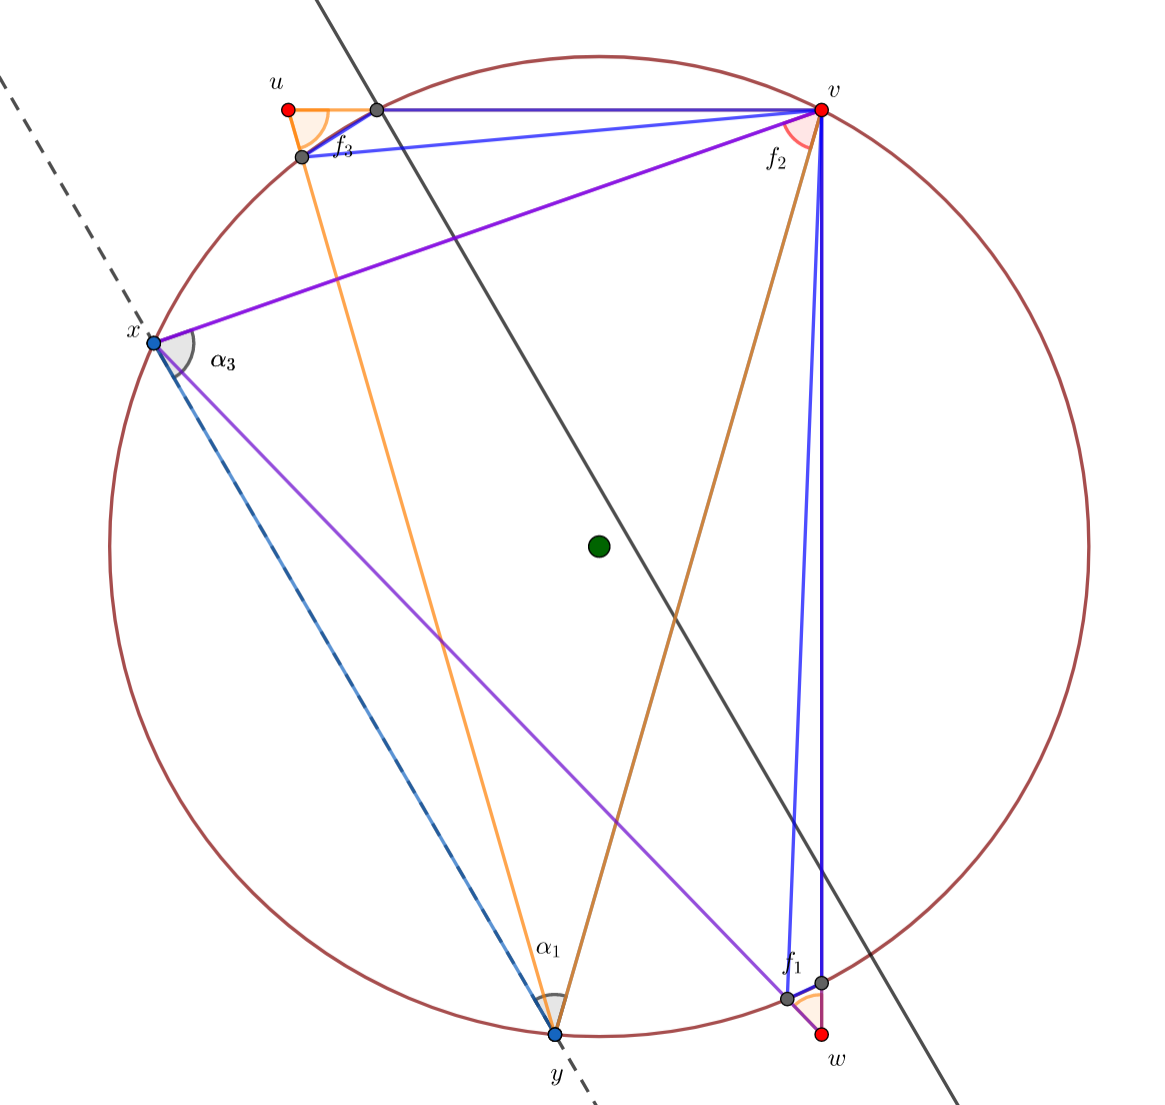
\includegraphics[width=.65 \paperwidth]{./images/Bosquejo14.png}
    %\caption*{.}
  \end{figure}
\end{frame}

\begin{frame}
  %\frametitle{Prueba.}
  \begin{figure}
    \centering
    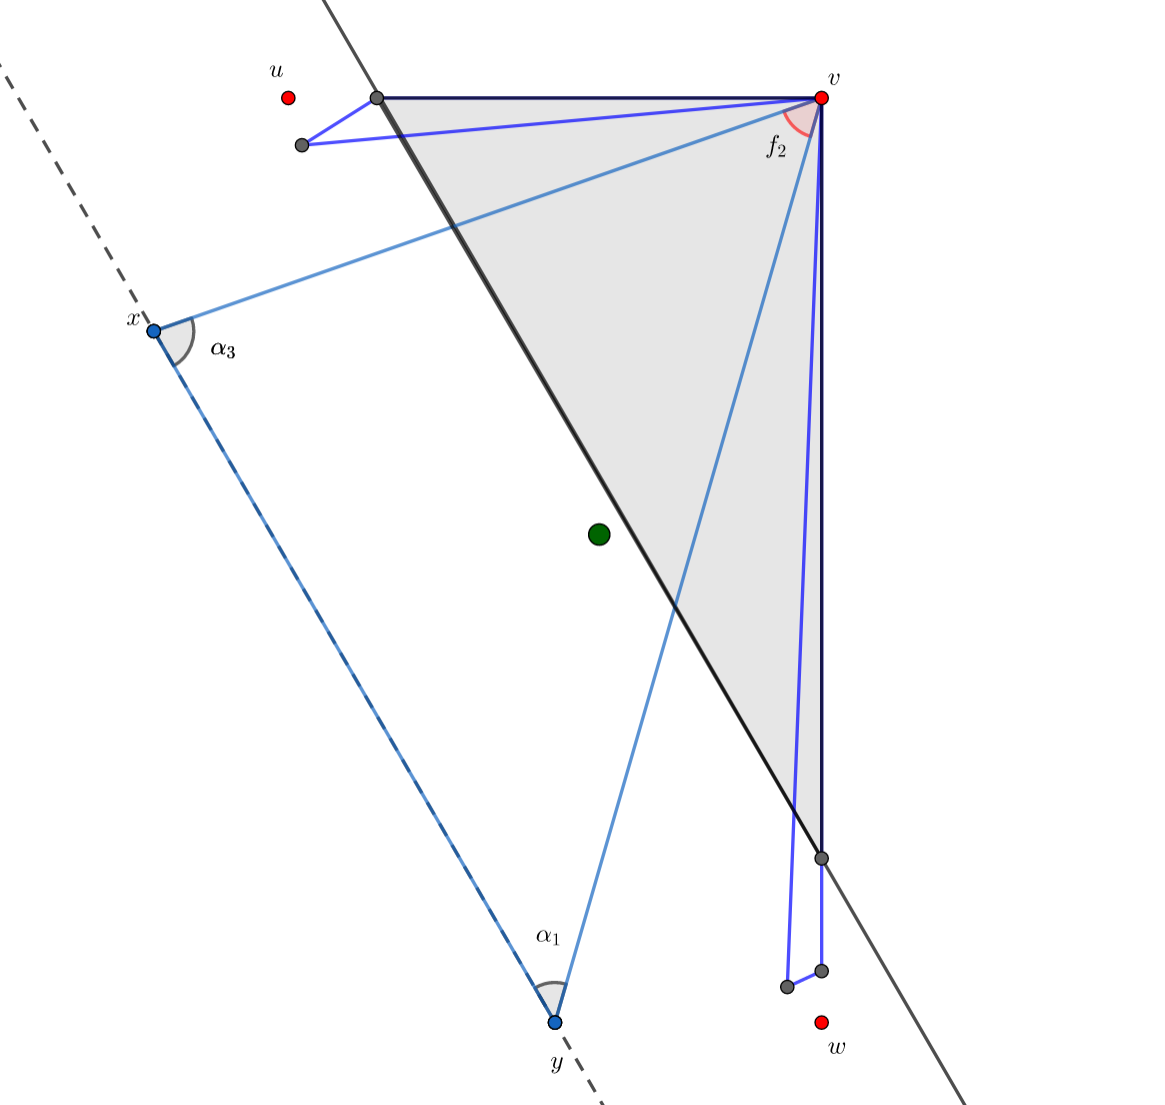
\includegraphics[width=.65 \paperwidth]{./images/Bosquejo15.png}
    %\caption*{.}
  \end{figure}
\end{frame}

\begin{frame}
  %\frametitle{Prueba.}
  \begin{figure}
    \centering
    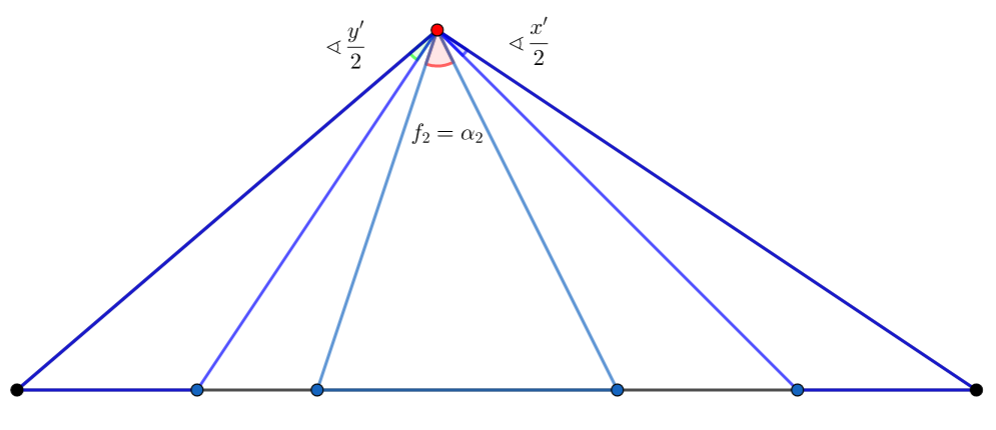
\includegraphics[width=.65 \paperwidth]{./images/D1.png}
    %\caption*{.}
  \end{figure}
\end{frame}

\begin{frame}
  %\frametitle{Prueba.}
  \begin{figure}
    \centering
    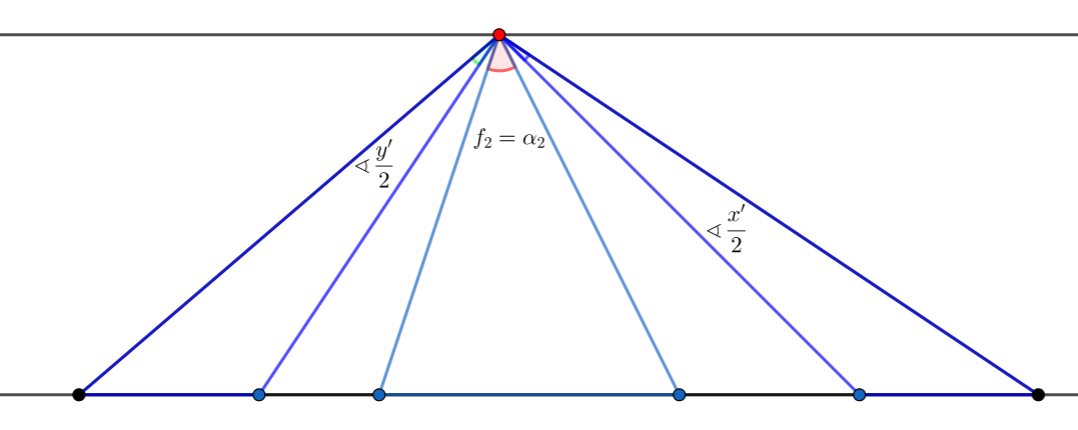
\includegraphics[width=.65 \paperwidth]{./images/D2.png}
    %\caption*{.}
  \end{figure}
\end{frame}

\begin{frame}
  %\frametitle{Prueba.}
  \begin{figure}
    \centering
    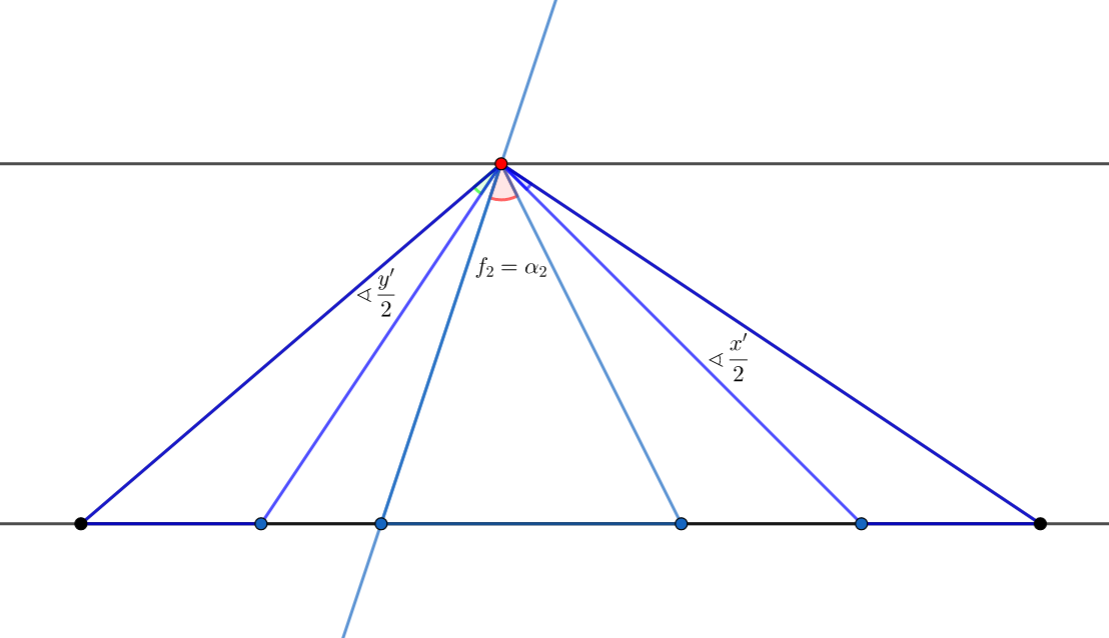
\includegraphics[width=.65 \paperwidth]{./images/D3.png}
    %\caption*{.}
  \end{figure}
\end{frame}

\begin{frame}
  %\frametitle{Prueba.}
  \begin{figure}
    \centering
    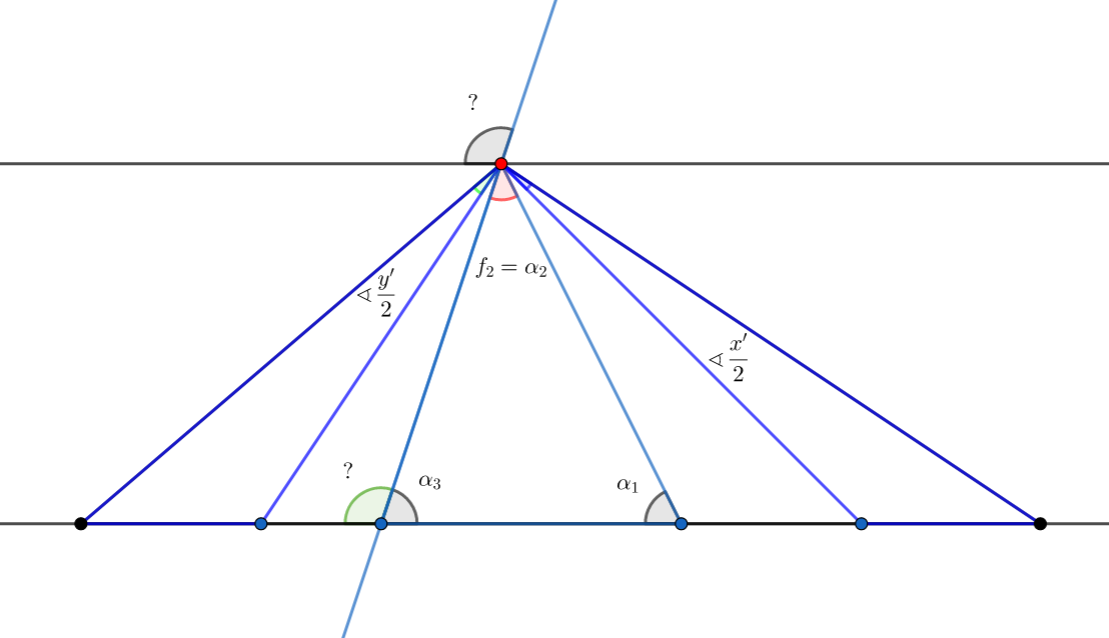
\includegraphics[width=.65 \paperwidth]{./images/D4.png}
    %\caption*{.}
  \end{figure}
\end{frame}

\begin{frame}
  %\frametitle{Prueba.}
  \begin{figure}
    \centering
    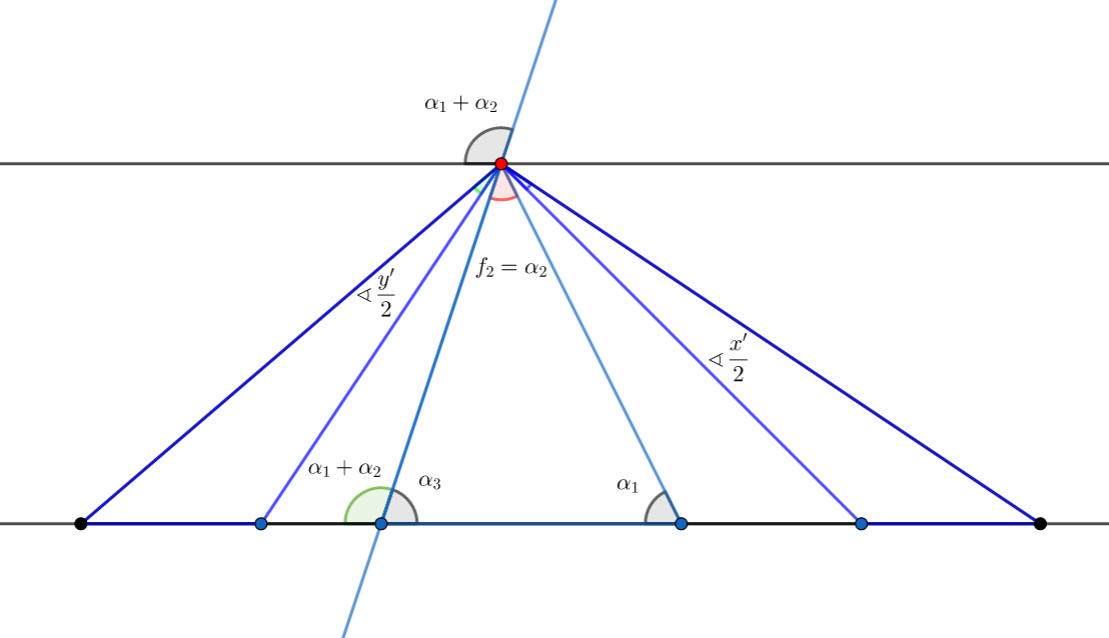
\includegraphics[width=.65 \paperwidth]{./images/D5.png}
    %\caption*{.}
  \end{figure}
\end{frame}

\begin{frame}
  \frametitle{Cuentas ...}
  Esto implica que
  \begin{eqnarray*}
    \sphericalangle \frac{x'}{2} &<& \alpha_1\\
    \sphericalangle \frac{y'}{2} &<& \alpha_3
  \end{eqnarray*}
  Luego, tenemos que
 \begin{eqnarray*}
   f_1 + f_3 &=& \alpha_1 + \alpha_3 - \frac{\sphericalangle x' + \sphericalangle y'}{2}\\
             &\leq& \alpha_1 + \alpha_3
 \end{eqnarray*}
 Por lo anterior, tenemos que
 \begin{eqnarray*}
   f_1 + f_2 + f_3 &\leq& \alpha_1 + \alpha_ 2+ \alpha_3.
 \end{eqnarray*}
\end{frame} 

\begin{frame}
  \frametitle{Caso 2.}
  \begin{figure}
    \centering
    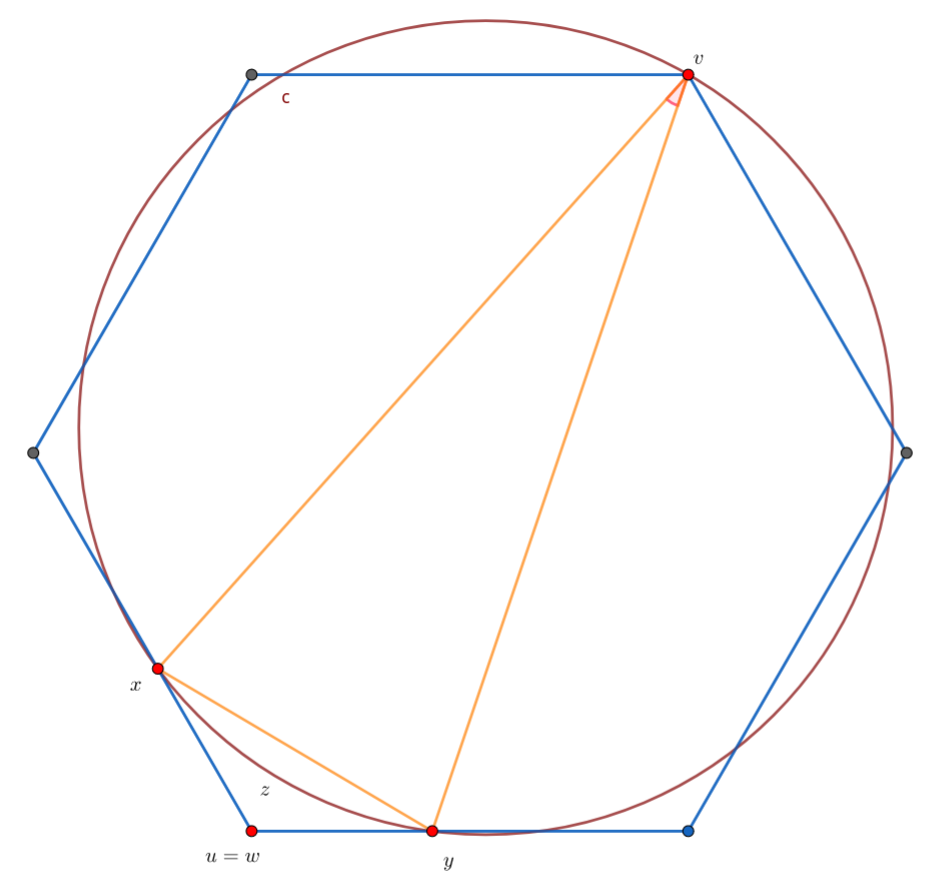
\includegraphics[width=.50 \paperwidth]{./images/Bosquejo16.png}
    %\caption*{.}
  \end{figure}
\end{frame}

\begin{frame}
  %\frametitle{Caso 2.}
  \begin{figure}
    \centering
    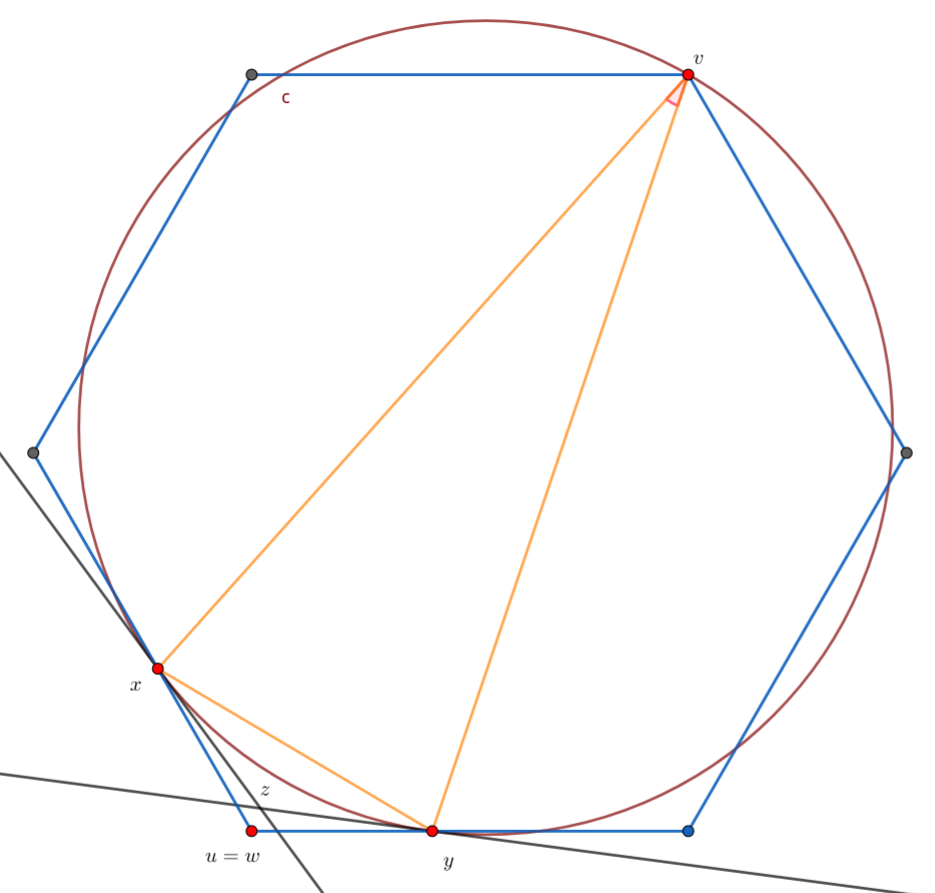
\includegraphics[width=.65 \paperwidth]{./images/Bosquejo17.png}
    %\caption*{.}
  \end{figure}
\end{frame}

\begin{frame}
  %\frametitle{Caso 2.}
  \begin{figure}
    \centering
    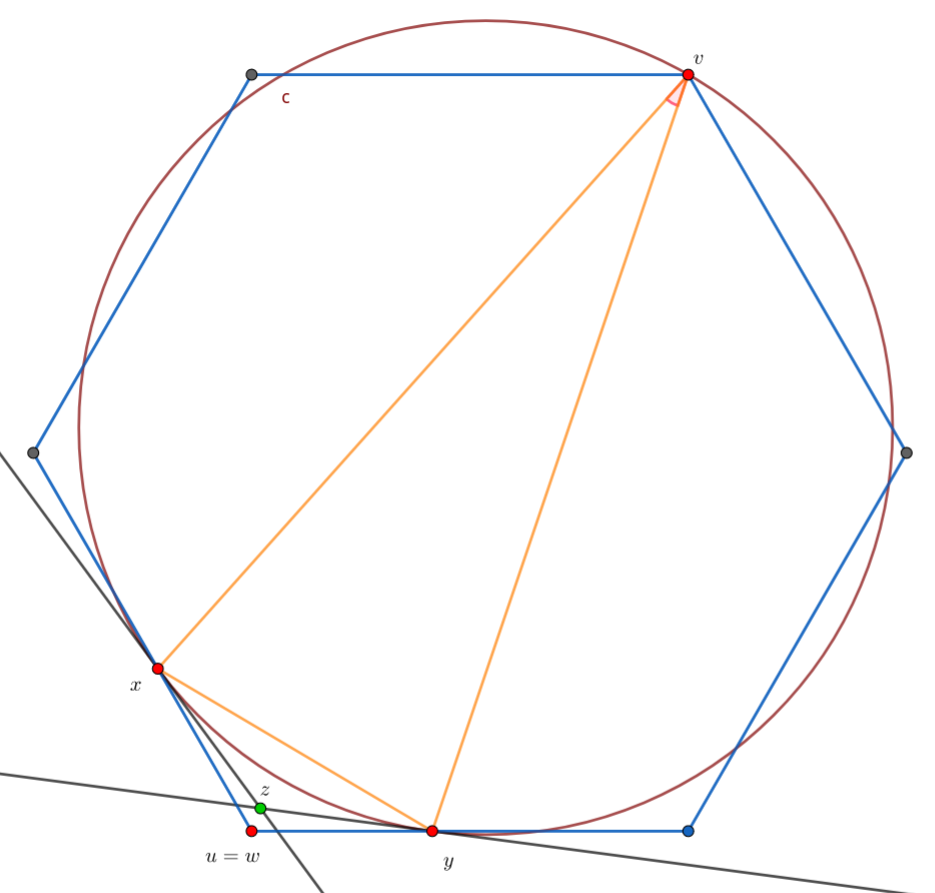
\includegraphics[width=.65 \paperwidth]{./images/Bosquejo18.png}
    %\caption*{.}
  \end{figure}
\end{frame}

\begin{frame}
  %\frametitle{Caso 2.}
  \begin{figure}
    \centering
    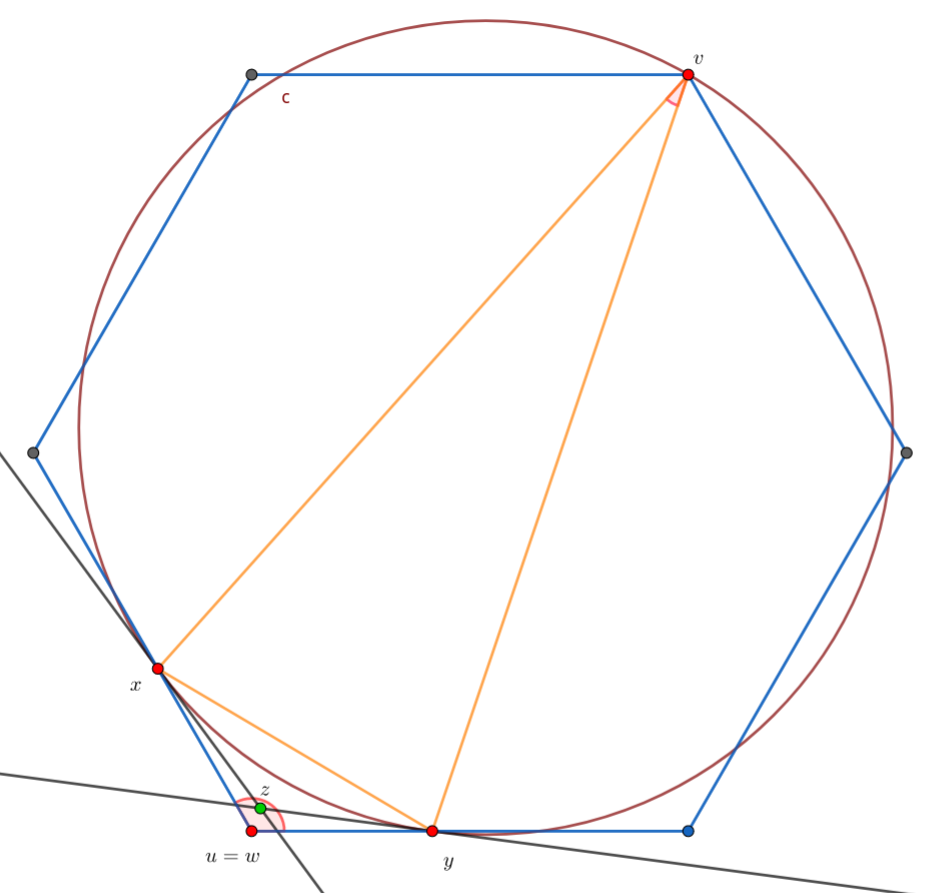
\includegraphics[width=.65 \paperwidth]{./images/Bosquejo19.png}
    %\caption*{.}
  \end{figure}
\end{frame} 

\begin{frame}
  \frametitle{Cuentas ...}
  De lo anterior tenemos que
  \begin{eqnarray*}
    \sphericalangle z &=& \frac{(2\pi - 2\alpha_2) - 2\alpha_2}{2}\\
                      &=& \frac{2\pi - 4\alpha_2}{2}\\
                      &=& \pi - 2\alpha_2\\
    \Rightarrow \sphericalangle w = \alpha_3 &<& \pi - 2\alpha_2\\
    \Rightarrow \alpha_2 + \alpha_3 &<& \pi - \alpha_2\\
    \Rightarrow \alpha_1 + \alpha_2 + \alpha_3 &<& \pi - (\alpha_2 + \alpha_1) \leq \pi.
  \end{eqnarray*}
  \hfill $\square$
\end{frame} 
